\begin{figure}[H]
\begin{center}
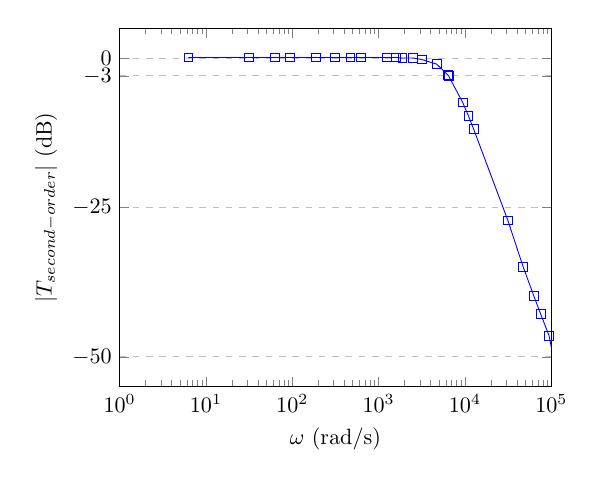
\begin{tikzpicture} [scale=0.8]
\begin{semilogxaxis}[
    title={},
    xlabel={$\omega$ (rad/s)},
    ylabel={$|T_{second-order}|$ (dB)},
    xmin=1, xmax=100000,
    ymin=-55, ymax=5,
    xtick={1,10,100,1000,10000,100000,1000000},
    ytick={0, -3, -25, -50},
    legend pos=north west,
    ymajorgrids=true,
    grid style=dashed,
]
\addplot[
    color=blue,
    mark=square,
    ]
    coordinates {
    (6.28,0.086)
    (31.42,0.086)
    (62.83,0.086)
    (94.25,0.086)
    (188.5,0.086)
    (314.16,0.086)
    (471.24,0.086)
    (628.32,0.086)
    (1256.64,0.086)
    (1570.80,0.086)
    (1884.96,0)
    (2513.27,0)
    (3141.59,-0.244)
    (4712.39,-1.031)
    (6283.19,-2.796)
    (6477.96,-3.012)
    (9424.78,-7.447)
    (10995.57,-9.710)
    (12566.37,-11.843)
    (31415.93,-27.171)
    (47123.89,-34.895)
    (62831.85,-39.830)
    (75398.22,-42.844)
    (94247.78,-46.462)
    (113097.34,-52.197)
    (125663.71,-54.420)
    };
\end{semilogxaxis}
\end{tikzpicture}
\hspace{1cm}
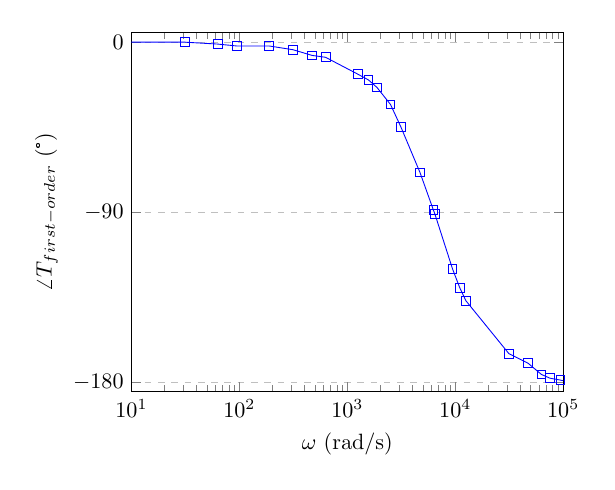
\begin{tikzpicture} [scale=0.8]
\begin{semilogxaxis}[
    title={},
    xlabel={$\omega$ (rad/s)},
    ylabel={$\angle T_{first-order}$ (°)},
    xmin=10, xmax=100000,
    ymin=-185, ymax=5,
    xtick={10,100,1000,10000,100000,1000000},
    ytick={0, -90, -180},
    legend pos=north west,
    ymajorgrids=true,
    grid style=dashed,
]
\addplot[
    color=blue,
    mark=square,
    ]
    coordinates {
    (6.28,0)
    (31.42,0)
    (62.83,-1)
    (94.25,-2)
    (188.5,-2)
    (314.16,-4)
    (471.24,-7)
    (628.32,-8)
    (1256.64,-17)
    (1570.80,-20)
    (1884.96,-24)
    (2513.27,-33)
    (3141.59,-45)
    (4712.39,-69)
    (6283.19,-89)
    (6477.96,-91)
    (9424.78,-120)
    (10995.57,-130)
    (12566.37,-137)
    (31415.93,-165)
    (47123.89,-170)
    (62831.85,-176)
    (75398.22,-178)
    (94247.78,-179)
    (113097.34,-180)
    (125663.71,-180)
    };
\end{semilogxaxis}
\end{tikzpicture}
\end{center}
\caption{Curvas de bode com os resultados práticos da função de transferência do filtro passa-baixas de 2ª ordem}
\label{graph:2} 
\end{figure}